
\chapter{Versuch}

\section{Ziel der Arbeit}

Das Ziel der Arbeit ist es, implizite Löser für Neuralodes zu verwenden 
und deren Performance anhand von Meshgraphnetzen zu evaluieren. 
Diese verwendet Neuralodes zur Simulation von Flüssigkeiten um verschiedene Körper in 2D.
Die Simulation basiert auf den Differenzialgleichungen, die das verhalten von Flüssigkeiten beschreiben.
Diese Gleichungen wurden nun verwendet, um das neuronale Netz der Neuralode zu trainieren.

% Nun können verschiedene numerischen Verfahren verwendet werden, um die Neuralode auszuwerten.
Anschließend können verschiedene numerische Verfahren verwdent werden, um das Netz auszuwerten.

Die Qualität des Ergebnisses kann dann mit den klassisch durchgeführten Differenzialgleichungen verglichen werden.
Da diese Berechnungen sehr lange dauern, ist es erstrebenswert, diese auf der GPU auszuführen.
Implizit und Explicit Löser von Anfangswerteproblemen laufen auf der CPU problemlos.
Das verwenden von impliziten Lösern auf der GPU führt allerdings zu Problemen, da für diese Automatik Differenziation durchgeführt werden muss.
Um die Ableitung verschachtelter Funktionen berechnen zu können, verwenden
Programme die AutomaticDifferentiation durchführen, Dualzahlen, welche von unserer Neuralode nicht unterstützt werden.
Das Problem dabei ist das, die Operation scatter innerhalb der Neuralode dual zahlen nicht auf der GPU 
berechnen kann.
Die scatter-Funktion um schnell die Änderungen eines Zeitschrittes auf alle Knoten im Netz anzuwenden.



\section{Implementierung der Scatter funktion}

Um unsere Neuralode auswerten zu können, müssen alle Teile der Differenzialgleichung Dual zahlen unterstützen.
In diesem Fall unterstützt die scatter-function von Flux nicht die Addition von Dual zahlen.
Die scatter Funktion ist wie folgt definiert:

\begin{lstlisting}{language=Julia}
	scatter(op, src, idx; [init, dstsize])
\end{lstlisting}

\begin{verbatim}
	op ist die operation die auf alle werte die in die selbe zelle geschrieben werden angewendet wird.
		mögliche werte sind +, -, *, /, min, max, mean
	src ist eine beliebige matrix aus der wert gelesen und wieder an anderer stelle zurück geschrieben werden.
	idx ist ebenfalls eine beliebige matrix aus der entnommen wird an welche position, der wert einer zelle geschrieben werden soll.
	init beschreibt wie das ziel array initialisiert wird.
			dies kann zum beispiel genutzt werden, um den inhalt des arrays in das geschrieben wird initial auf null zu setzten.
	dstsize gibt die größe des zurück gegebenen arrays an.
\end{verbatim}

Aus der Definition wird nicht ganz klar, was mit dem Ziel Array gemeint ist.
Um dies besser verstehen zu können, wird eine vereinfachte Version der Implementierung der scatter Funktion betrachtet.

\begin{lstlisting}{language=Julia}
	function scatter(op, src, idx; [init, dstsize])
		dst = similar(src)
		
		fill!(dst, init)
		
		scatter!(op, dst, src, idx)
	end
\end{lstlisting}

Die scatter Funktion erstellt zuerst ein Array vom selben Datentype und der benötigten Größe. 
Wie die Größe berechnet wird, wurde hier weggelassen, da dies für unsere Zwecke nicht relevant ist. 
Anschließend wird das dst Array mit den gewünschten Initial werten gefüllt.
Als Letztes wird nun die scatter! Funktion aufgerufen.
Das Ausrufezeichen im Funktionsnamen symbolisiert, das die Funktion, die Werte der übergebenen Argumente überschreibt.
Die scatter! Funktion wird in diesem Fall von der NNlibCUDA Bibliothek überschrieben und sorgt dafür, 
dass die Berechnung auf der Grafikkarte ausgeführt wird.
Die Grafikkarte führt dabei in mehrer Threads die Operation op aus. In unserem Fall ist op die + Funktion.
Dabei kann es passieren, dass mehrere Threads zum gleichen Zeitpunkt in dasselbe Feld schreiben.
Normaler weiße kommt es dabei zu einer viel zahl von Fehler, wenn keine Sicherheit maßnahmen getroffen werden. 
Da dies ein sehr häufiges Problem bei Berechnungen ist, bietet die CUDA-libarary, 
welche verwendet wird, um die Berechnungen auf der Grafikkarte auszuführen atomic-operationen an
welche genau diese Fehler umgehen.
% https://docs.nvidia.com/cuda/cuda-c-programming-guide/index.html#atomic-functions
Das Problem dabei ist, dass diese Atomic-operationen nur auf 32-Bit oder 64-Bit Zahlen ausgeführt werden können.
Außerdem werden nur bestimmten Datentypen unterstützt.
Es ist zwar möglich, diese Operation auf weitere Datentypen zu erweitern, diese müssen aber kleiner als 64-Bit sein. 
Dies macht es für unsere Zwecke unmöglich, Dual zahlen mit dieser Operation direkt zu berechnen.
Da die Atomic-opertion von Cuda nicht direkt verwenden kann, muss eine anderer weg gefunden werden.
Um Dual Zahlen zu implementieren, wird dessen mathematisch definition betrachtet.

$$
d = a + b \epsilon \text{ wobei gilt } \epsilon^2 = 0
$$

Für die Definition von Dual-Zahlen ist ebenfalls ihr verhalten auf scalare Operationen wichtig:

$$
 f( a + b \epsilon ) = f(a) + b f'(x) \epsilon
$$

Um die scatter-function umzusetzen, wird die Definition der Addition benötigt.

$$
(a + b \epsilon) + ( c + d \epsilon ) = (a + c) + (b + d) \epsilon
$$

Die Definition von Dual zahlen kommt von der Addition komplexer Zahlen, 
da die Dual zahlen eine variante von generalisierten komplexen zahlen sind.
Zwei Dual zahlen werden addiert, indem die einzelnen Komponentern addiert werden.
Da die einzelnen Komponenten  alle Rellezahlen sind, lässt sich die auf der GPU durchführen.
Es kann also der @atmic call in der scatter! function durch folgende Implementierung ersetzt werden:

\begin{lstlisting}{language=Julia}

function gpu_add!(d0::Dual, d1::Dual, d2::Dual)
	@atomic value(d0) = value(d1) + value(d2)
	
	for i in 1:length(partials(d0))
		@atomic partials(d0, i) = partials(d1, i) + partials(d2, i)
	end
end

\end{lstlisting}

Wird die scatter Funktion nun wie beschrieben implementiert, kommt es zu einem weiteren Problem.
Der Macro @atomic verbietet die Funktions aufrufe value und partial.
Der Aufruf der partial-Funktion führt außerdem skalare Indexierung durch, welche auf der Grafikkarte nicht erlaubt ist.
Im Allgemeinen macht aber vor allem das Erstellen und zurück schreiben des Dual-structs große Probleme
da um dies durchzuführen, ebenfalls skalare Indizierung benötigt wird.
Prinzipiell ist es möglich, dieses Problem zu lösen, 
allerdings führt es zu sehr unübersichtlichen code, der sehr fehleranfällig ist, 
da große Teil der scatter Funktion mit minimalen Veränderungen wieder implementiert werden müssen.
Außerdem muss innerhalb des Kernels speicher reserviert werden, was zu Problemen bei großen Probleminstanzen führt.

\subsection{Eine Funktionierende Implementierung}

Bis her haben wir nun ansätze gesehen die aus unterschiedlichen gründen nicht funktionieren.
Eine elegante Lösung ergibt sich wenn, 
die scatter! function zur berechung der scatter! function verwendet wird.
Dies funktioniert indem die Fähigkeit der scatter function höher dimensinale daten auszuwerten, ausgenutzt wird. 
Es wird ein array mit dimension N das dual werte speichert in ein array von z.B Float mit der Dimension N+1 umgewandelt. 
In der Zusätzlichen Dimension werden die einzelnen Komponenten der Dual zahl abgespeichert.
Die größe der hinzugefügten dimension hängt, davon ab wie groß die partial componete der Dual zahl ist.
Um nun die addition um zusetzten, muss noch das index array der scatter function angepasst werden.
Dieses wird ebenfalls um eine dimension erweitert, und mit dem ziel index im src array erweitert.
Es werden also die zahlen von 1 bis n+1 in die zusätzliche dimension eingefügt.
Die folgende Graphik illustriert diesen vorgang in mit $N = 1$, der vorgang ist aber für höhere dimensionen analog

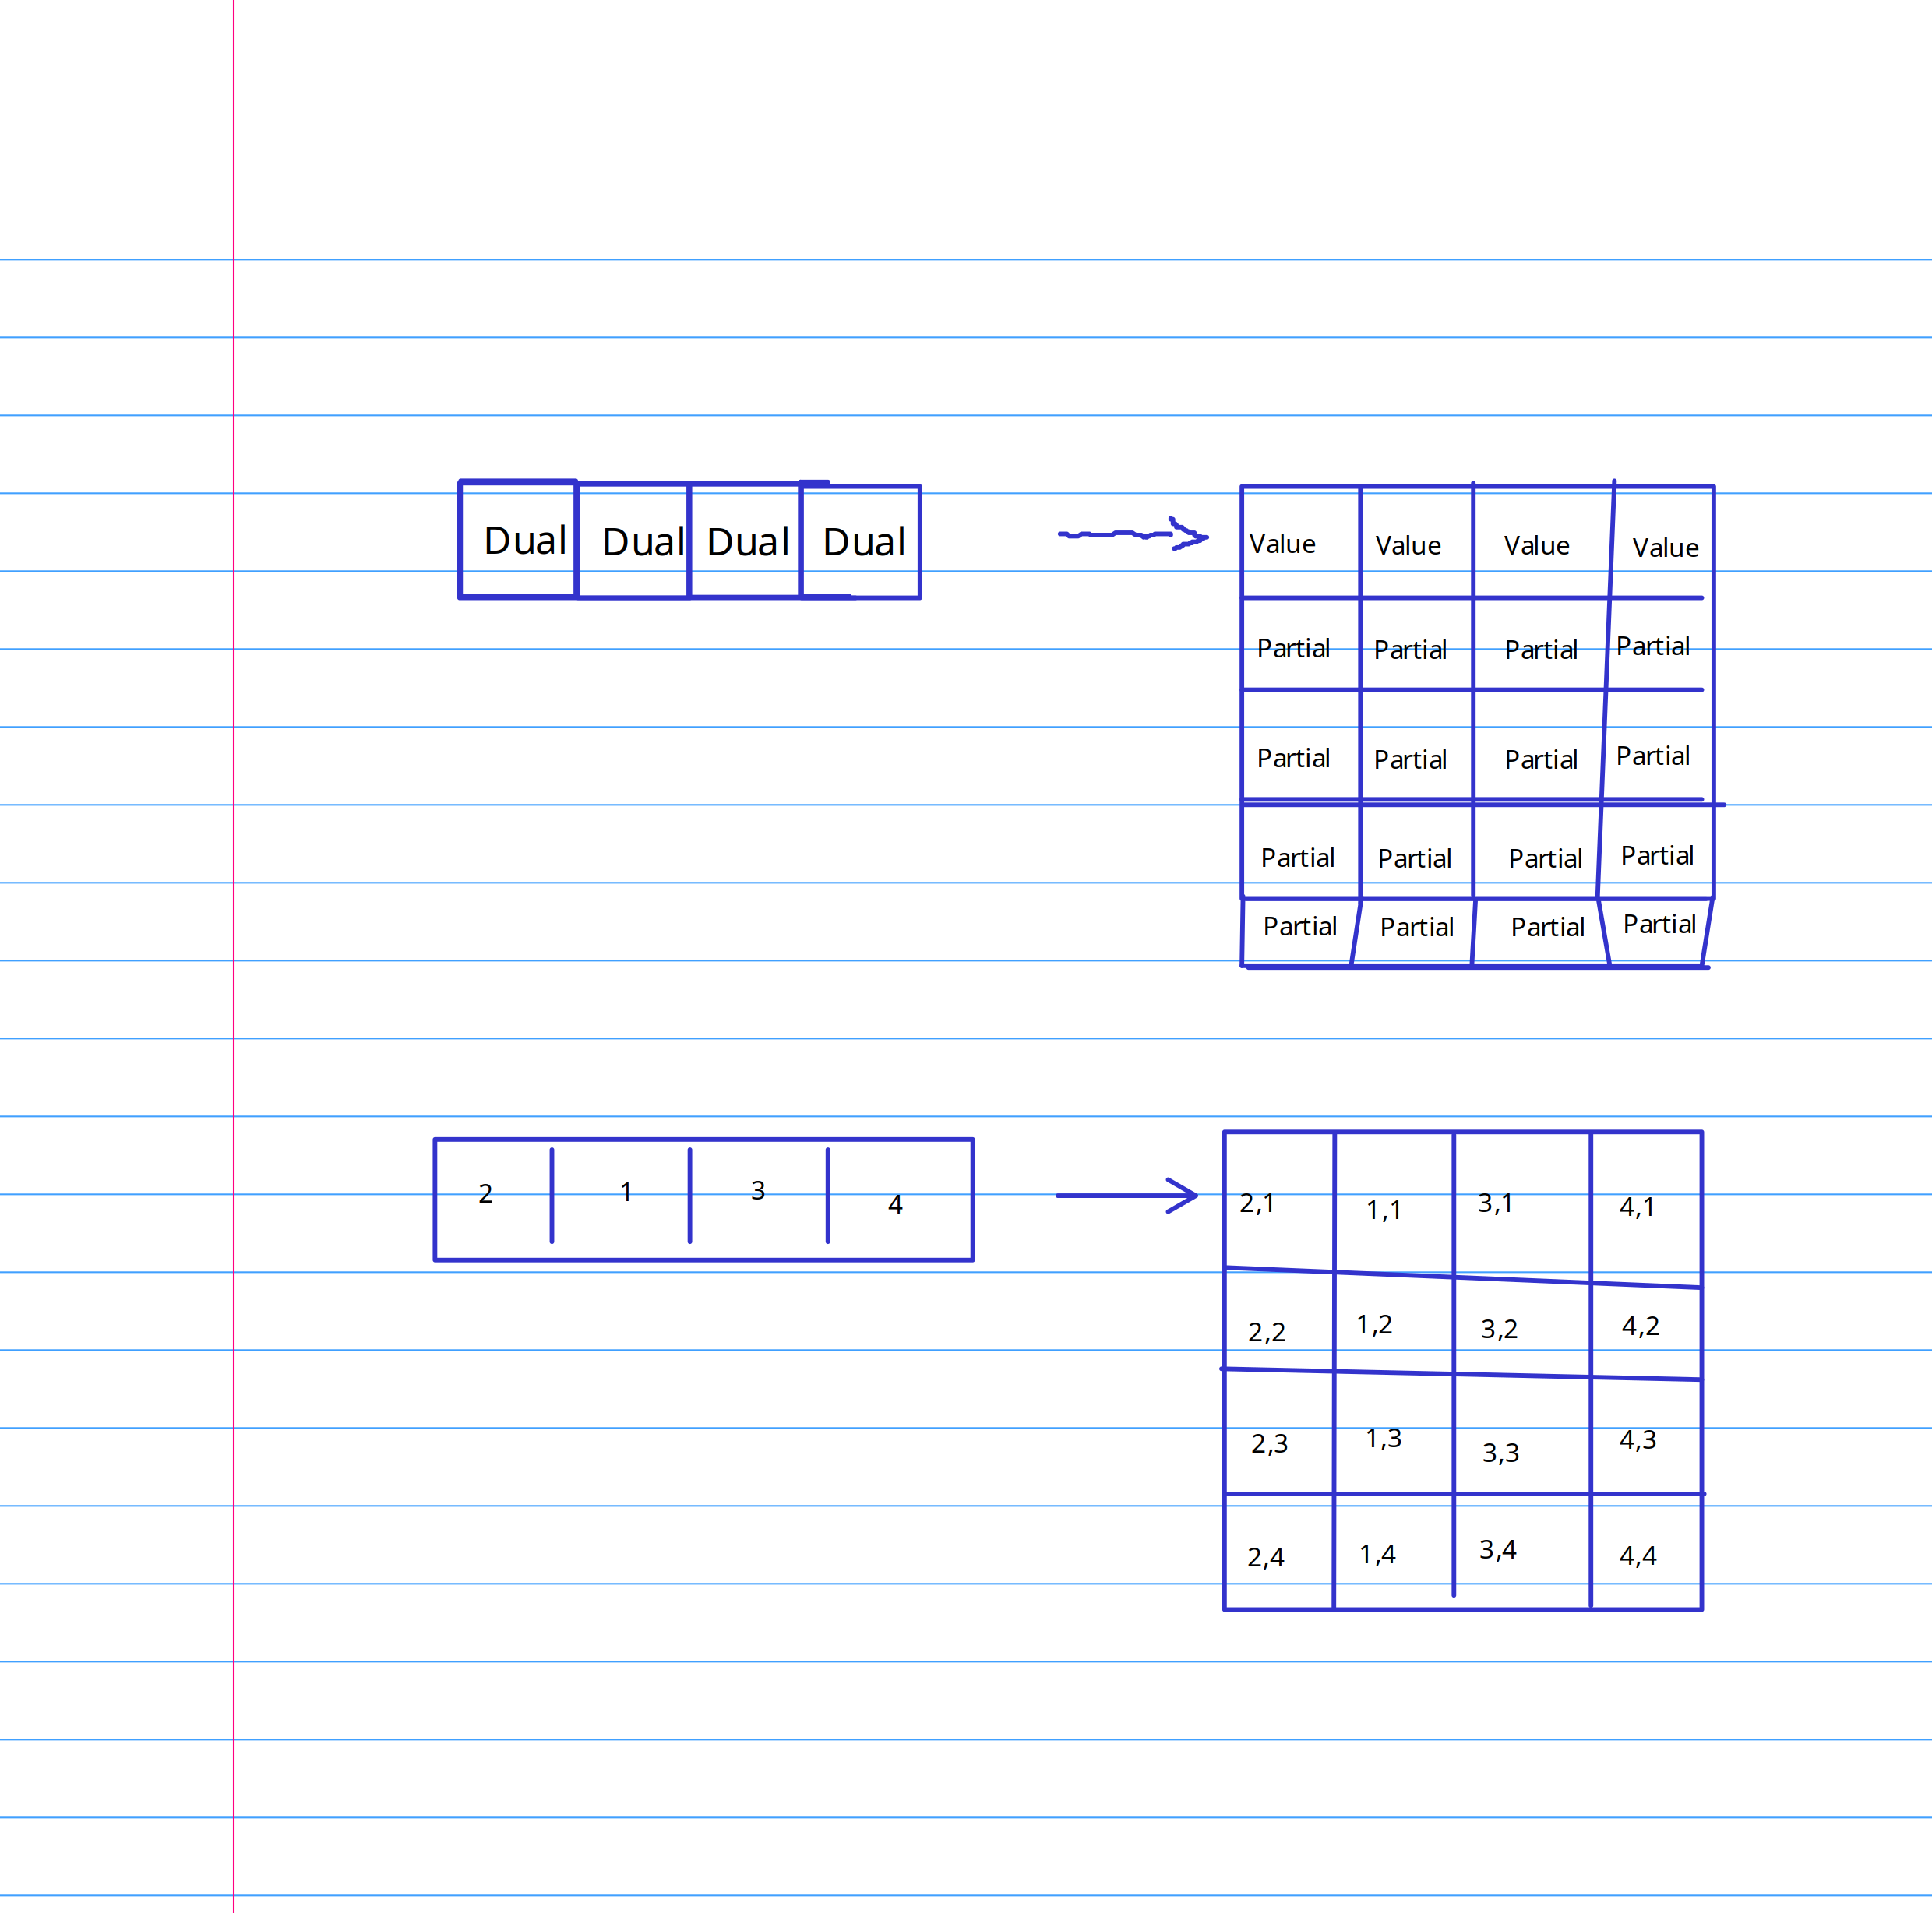
\includegraphics[width=\textwidth]{Data/02_Versuch/cropted.png}

Werden die veränderten arrays nun an die NNlibCUDA.scatter! function übergeben,
wird die scatter! operation auf dual-zahlen korrekt ausgeführt.
Zuguter letzt, muss nur noch das dual struct wieder konstruiert und in das ziel array zurück geschrieben werden. 
Dabei tritt nun das zuvor beschriebene problem der skalaren indezierung wieder auf.
Dieses Problem wirde gelößt indem, dem Kernel befor er gestartet wird nicht das array direkt, übergeben wird
sondern eine View auf dieses.
Eine view sorgt dafür das auf ein bestehndes array, anders zugeriffen werden kann.
Dies führt dazu das es nicht notwendig ist eine scalare operation auf das ziel array durch zuführen.
Der gesamte Process wird im folgendem nochmal genauer in pseudocode dargestellt.

\begin{verbatim}
	1. Allocate CUDA Memory 
		...		
		
	2. Copy the modified values into the allocated Memory
		...
		
	3. Call NNlib.scatter
		...
		
	4. Copy the result into the dst array
		...
\end{verbatim}


\section{ Fehler behebung in den Impliziten Lösern }

Da nun die scatter Funktion mit dual zahlen auf der GPU durchgeführt werden kann, 
sollte die Verwendung der Impliziten Löser nichts mehr im weg stehen.
Allerdings hat sich Julia im laufe der zeit weiter entwickelt und einig API Änderungen vorgenommen.
Dies hat auf der Seite der Löser dazu geführt, dass diese zum Teil Funktionalität von Julia 1.8 wollten und zum Teil Funktionalität von den früheren Versionen.
Das Problem war das sich die Implementierung der lu-factorisierung geändert hat.
In den älteren Versionen hat CUDA diese Implementierung selbst bereitgestellt.
Mit der Version 1.8 wurde dies allerdings in die Standard Bibliothek so aufgenommen, das die Faktorisierung 
auch auf der Grafik karte durchgeführt werden kann.
Das OrdenaryDifferentialEquations packet von Julia verwendet 
ein Array-Interface, welches operationen auf Arrays, 
von der Umsetzung abstrahiert, um diese auf einer Grafikkarte durchführen zu können.
Dank der Hilfe von Christopher Rackauckas ist es, dann nach vielen versuchen gelungen, die lu\_instance Funktion richtig umzusetzen 
und es damit möglich zu machen zumindest die im nächsten Kapitel vorgestellten impliziten Löser zum Laufen zubringen.











